\documentclass[10pt,a4paper]{article}
\usepackage[latin1]{inputenc}
\usepackage{amsmath}
\usepackage{amsfonts}
\usepackage{amssymb}
\usepackage{graphicx}
\begin{document}

\title{Topology of Particle Swarm}

\date{}

\maketitle

In the topology, there are three types of agents:
\begin{itemize}
\item particle
\item global best
\item person best
\end{itemize}

\begin{figure}[h]
\centering
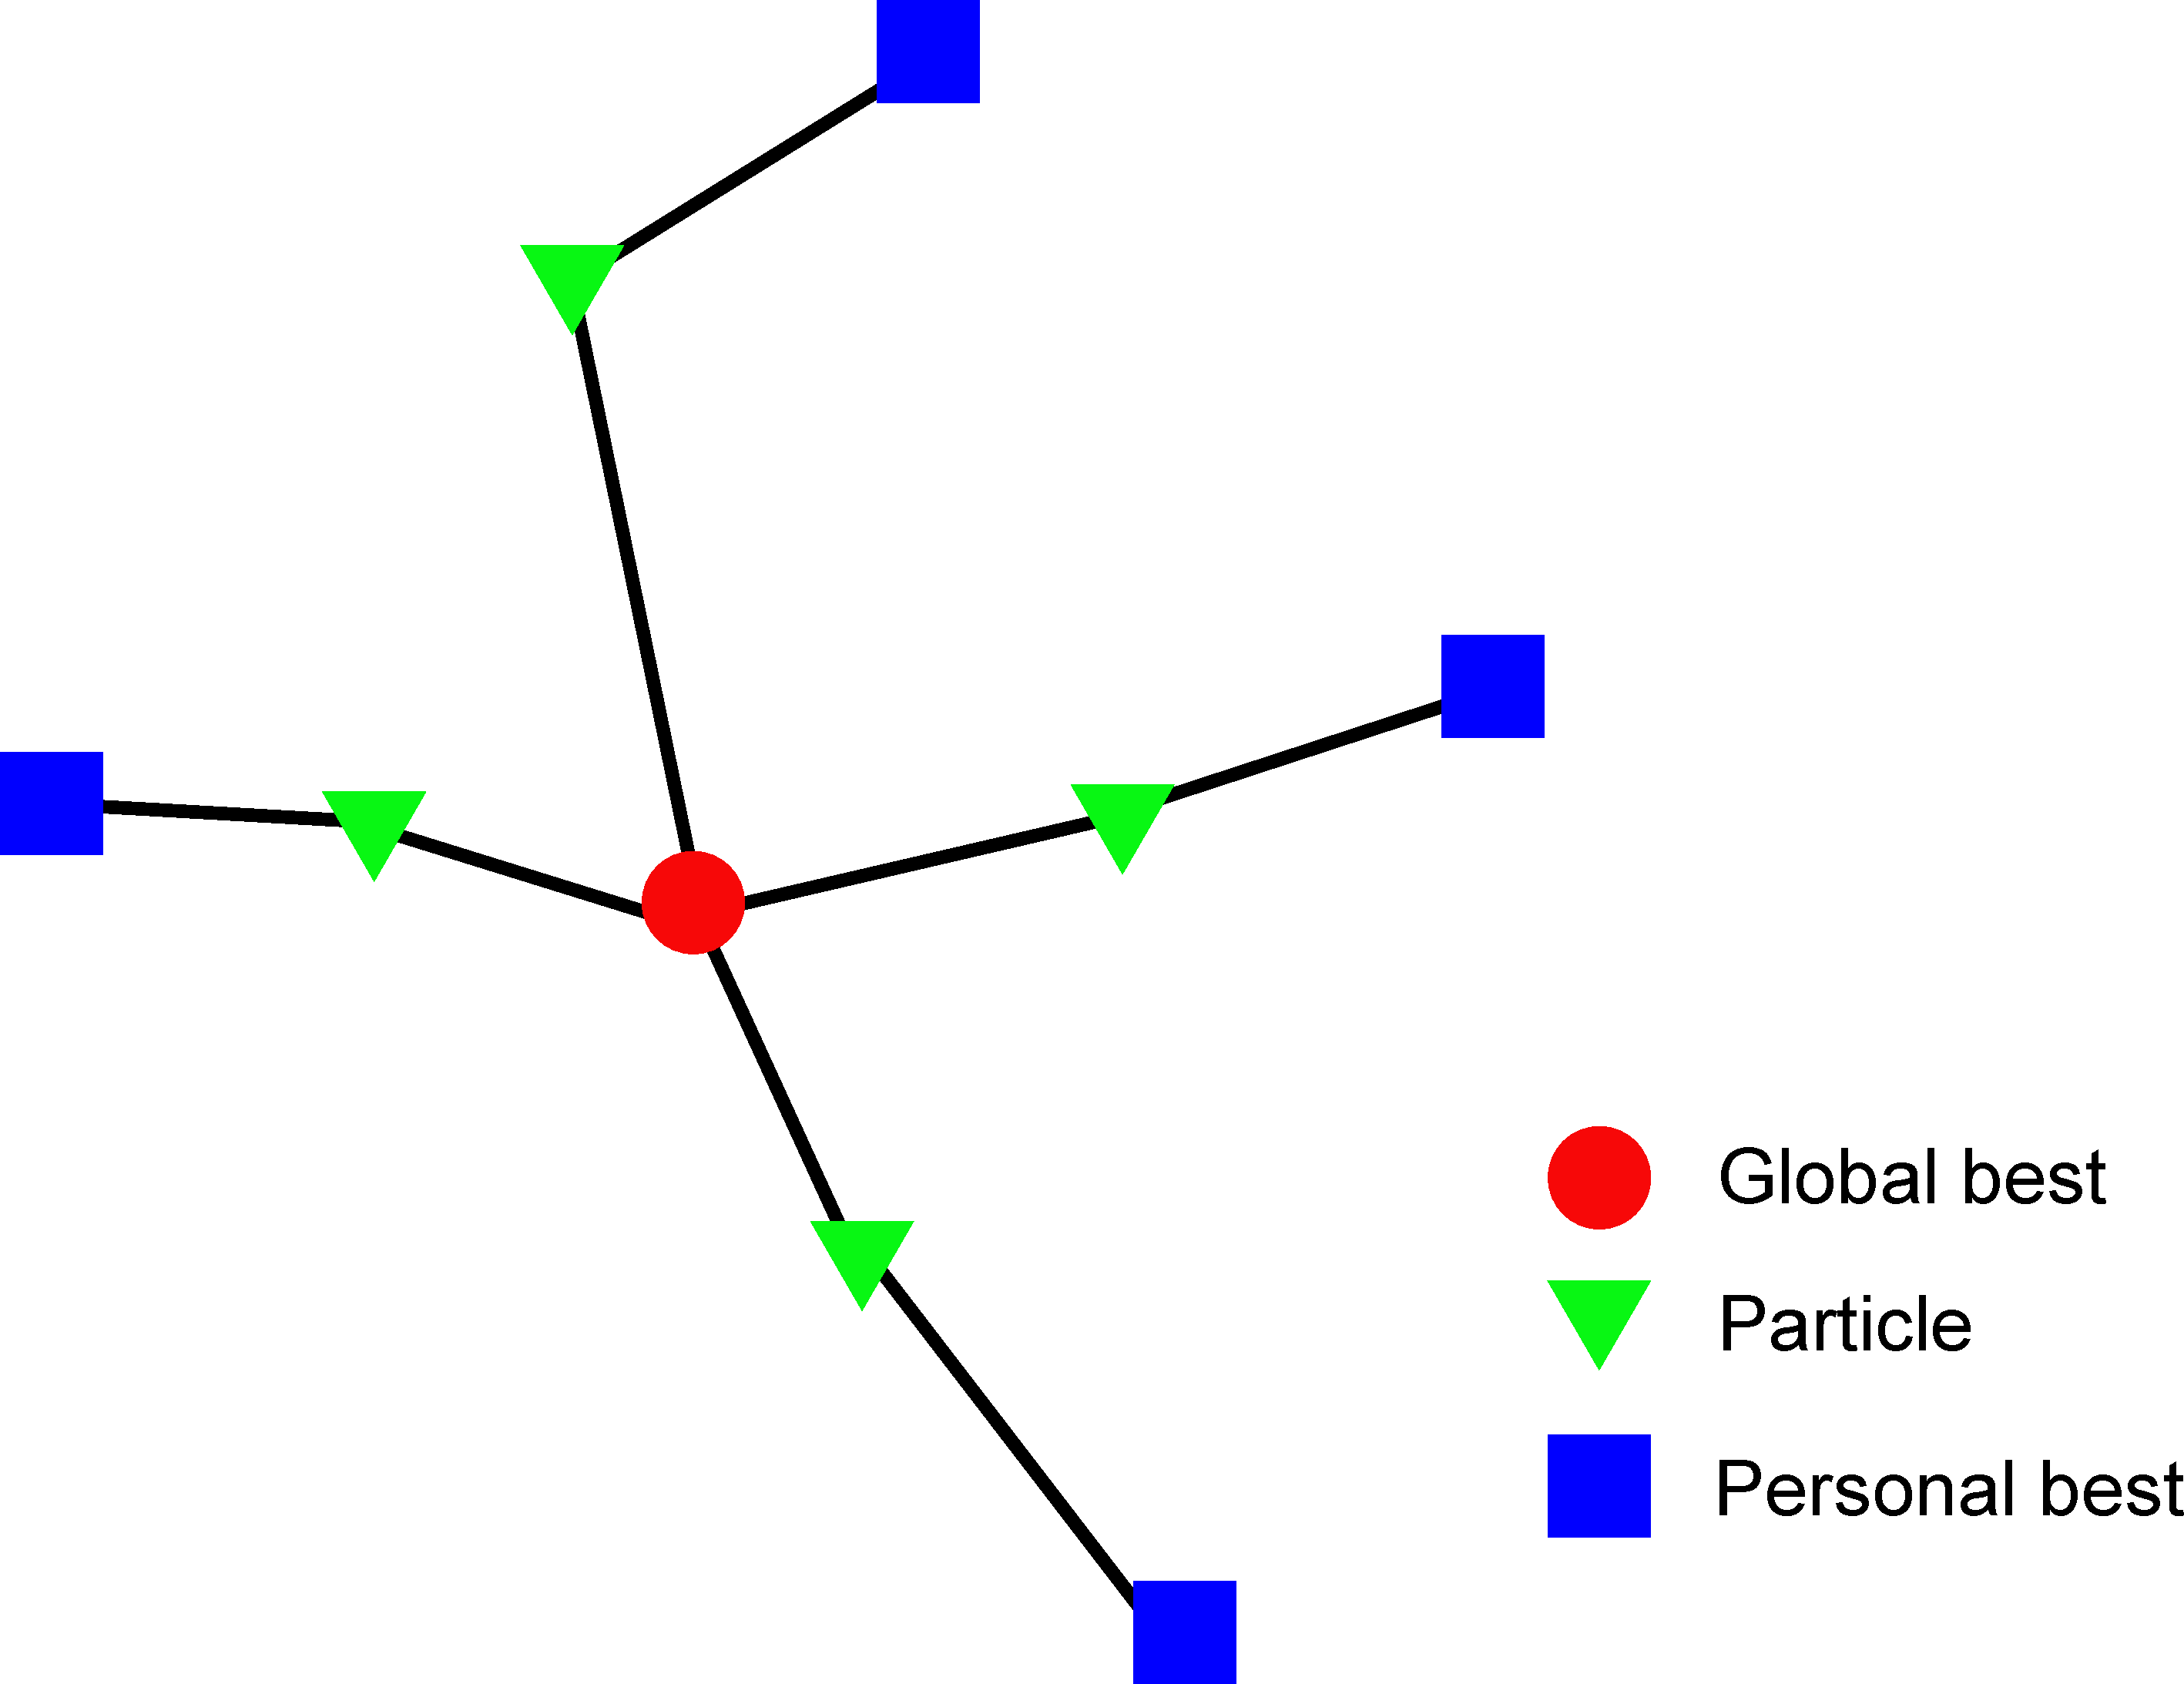
\includegraphics[width=0.7\linewidth]{topology}
\caption{The topology of the particle swarm}
\label{fig:topology}
\end{figure}

Different type of agents has different update rule.
The particles is 
\begin{equation}
x_{i} = \chi( \phi^{P} \sum_{ j \in N^{P} } ( x_{j} - x_{i} ) + \phi^{G} \sum_{ k \in N^{G} } ( x_{k} - x_{i} ) ),
\end{equation}
$ N^{G} $ is the set of neighboring global best, $ N^{P} $ is the set of neighboring personal best.
The personal best and the global best is
\begin{equation}
x_{i} = \arg \, \max_{ j \in N } ( f( x_{i} ) , f( x_{j} ) )
\end{equation},
$ N $ is the set of all neighbors.

We are interested with the synchronization of this system.
It looks like that the update rule of the personal best and the global best is not always convergent, which maybe depend on how the fitness space is like.

Currently we only focus on the convergence in the solution space.
If we look at the fitness space, the personal best agent and the global best agent should have convergent properties.
\begin{equation}
f( x_{i} ) = f( \arg \, \max_{ j \in N } ( f( x_{i} ) , f( x_{j} ) ) ) = \max_{ j \in N } ( f( x_{i} ) , f( x_{j} ) )
\end{equation}
For the particle agent, if $ x_{i} $ is stable in solution space, $ f( x_{i} ) $ should also be stable in fitness space.
I am guessing that we could utilize these to arrive a convergence proof in the fitness space.

\begin{figure}
\centering
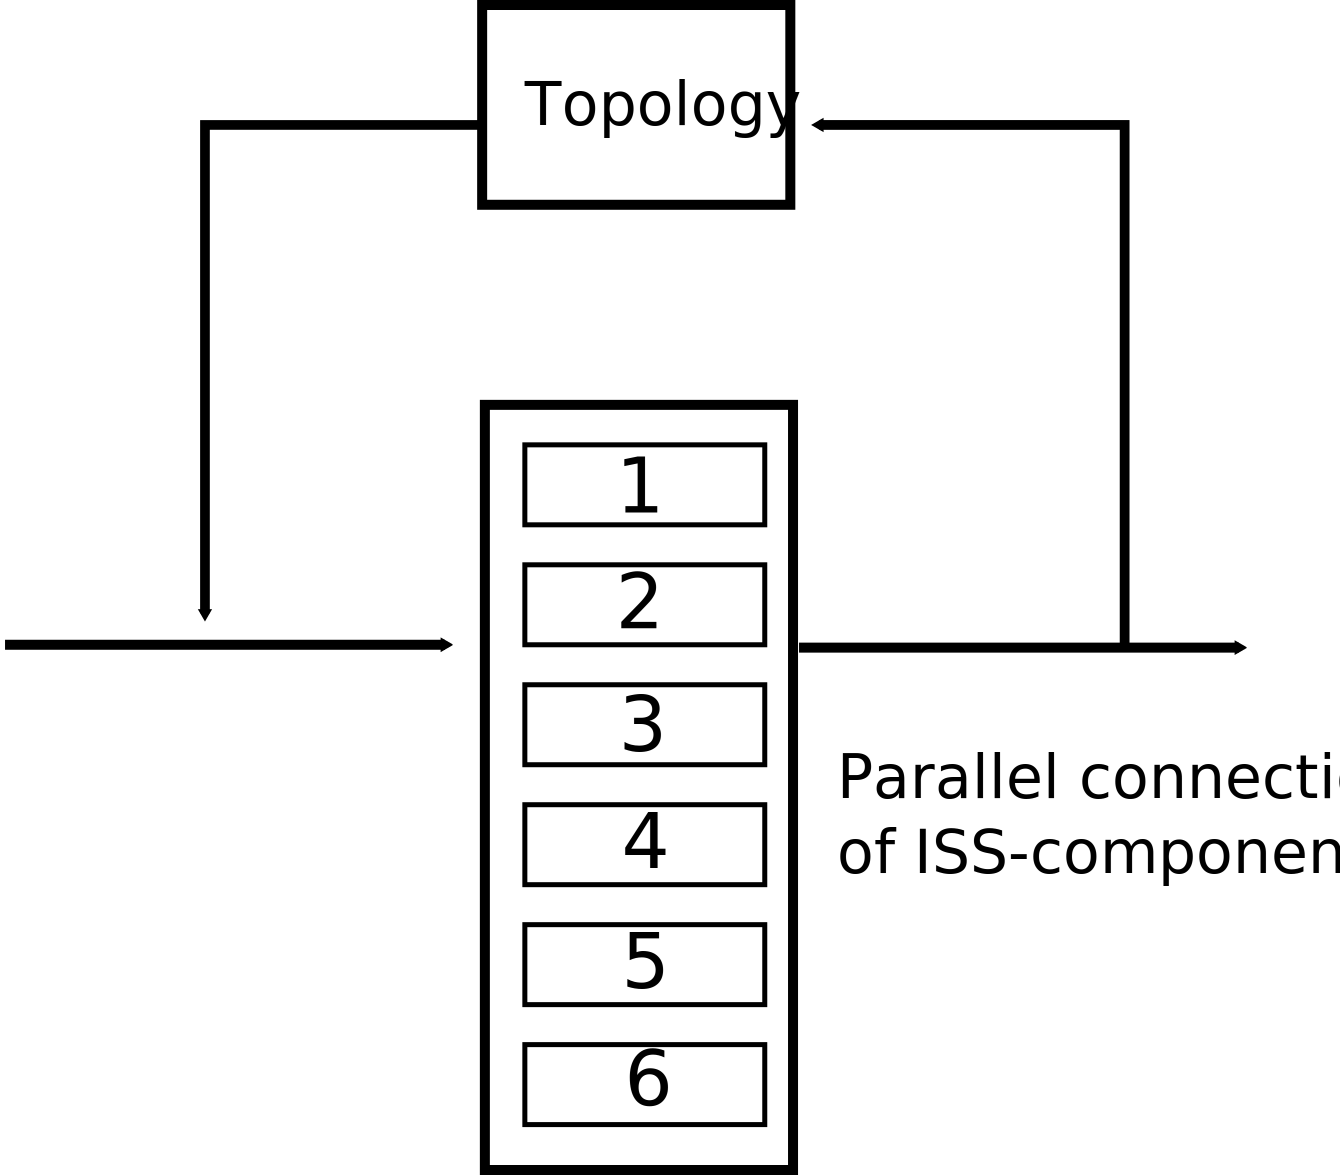
\includegraphics[width=0.6\linewidth]{./iss_structure}
\caption{A hypothesis on a ISS-connected stable struture.}
\label{fig:iss_structure}
\end{figure}

A parallel connection of ISS component still reserve the ISS.
The hypothesis is that when the topology satisfies some condition, it will make the system a stable one.

If we ignore the swarm topology, a particle can be viewed as in Figure \ref{fig:particle_topology}.

\begin{figure}
\centering
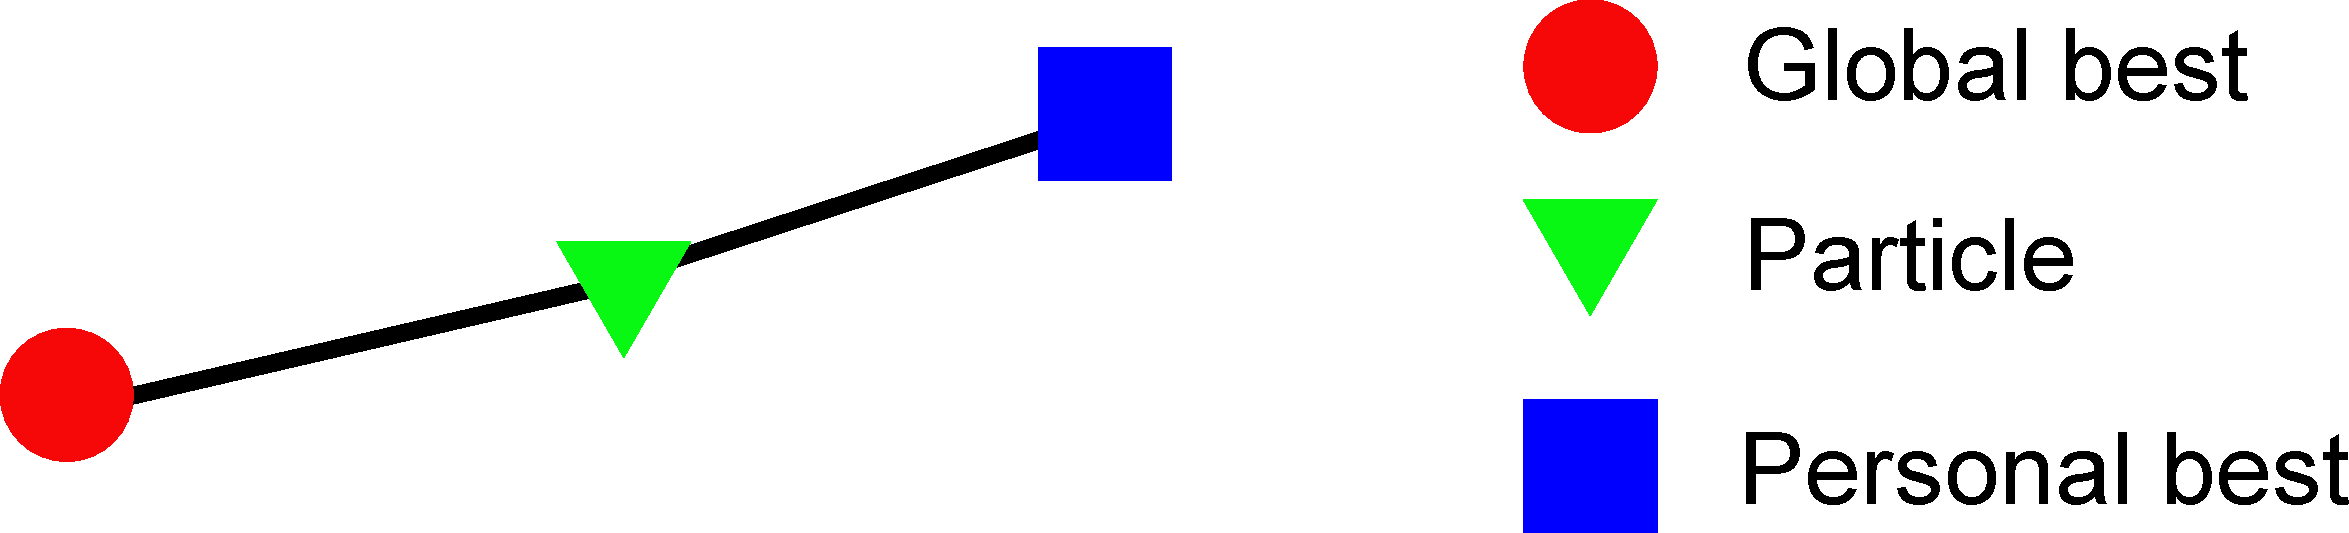
\includegraphics[width=0.7\linewidth]{./particle_topology}
\caption{A particle-wide topology.}
\label{fig:particle_topology}
\end{figure}

In stagnation, it means that the global best agent and the personal best agent become static (not moving).
We probably can do case analysis using the current conclusion on the ISS property of a particle.
I feel no matter how the fitness surface is like, there are only two patterns, which are one hill pattern (Figure \ref{fig:one_hill_case}) and two hills pattern (Figure \ref{fig:two_hills_case}).

\begin{figure}[h]
\centering
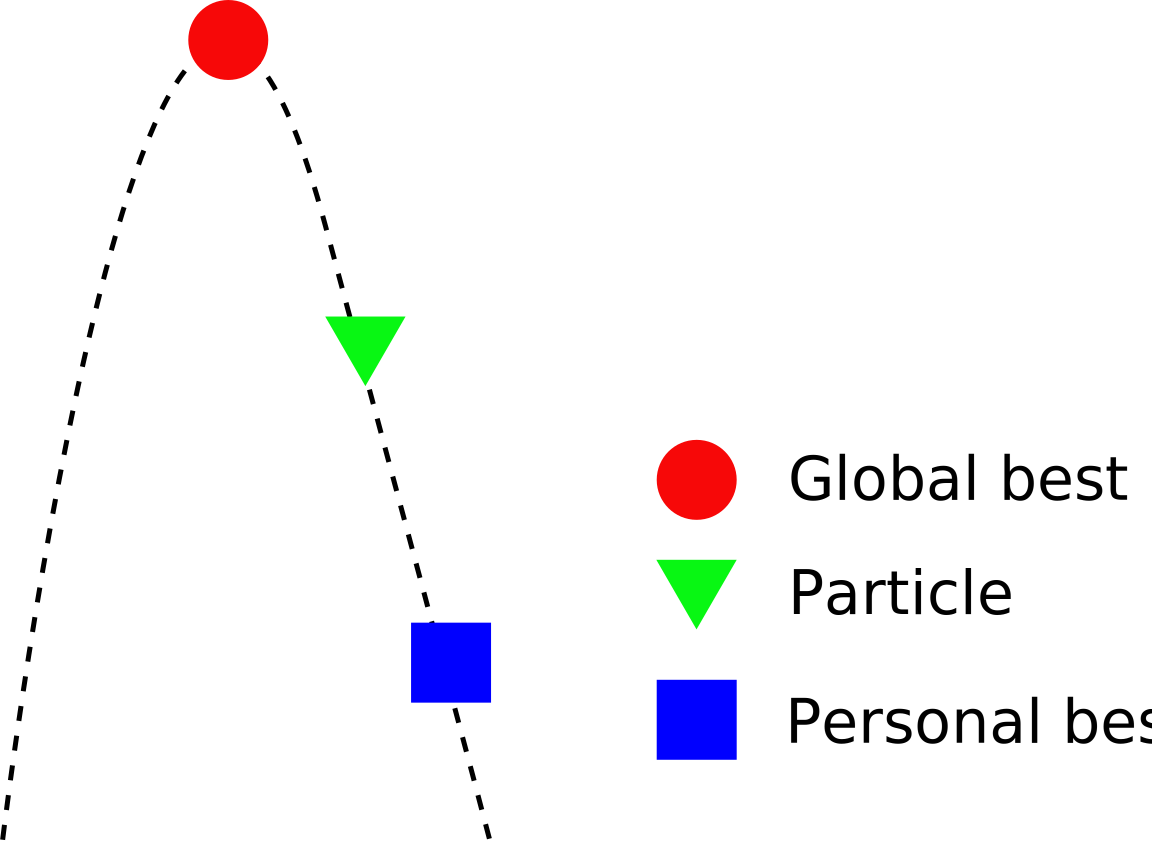
\includegraphics[width=0.5\linewidth]{./one_hill_case}
\caption{One hill case}
\label{fig:one_hill_case}
\end{figure}

\begin{figure}[h]
\centering
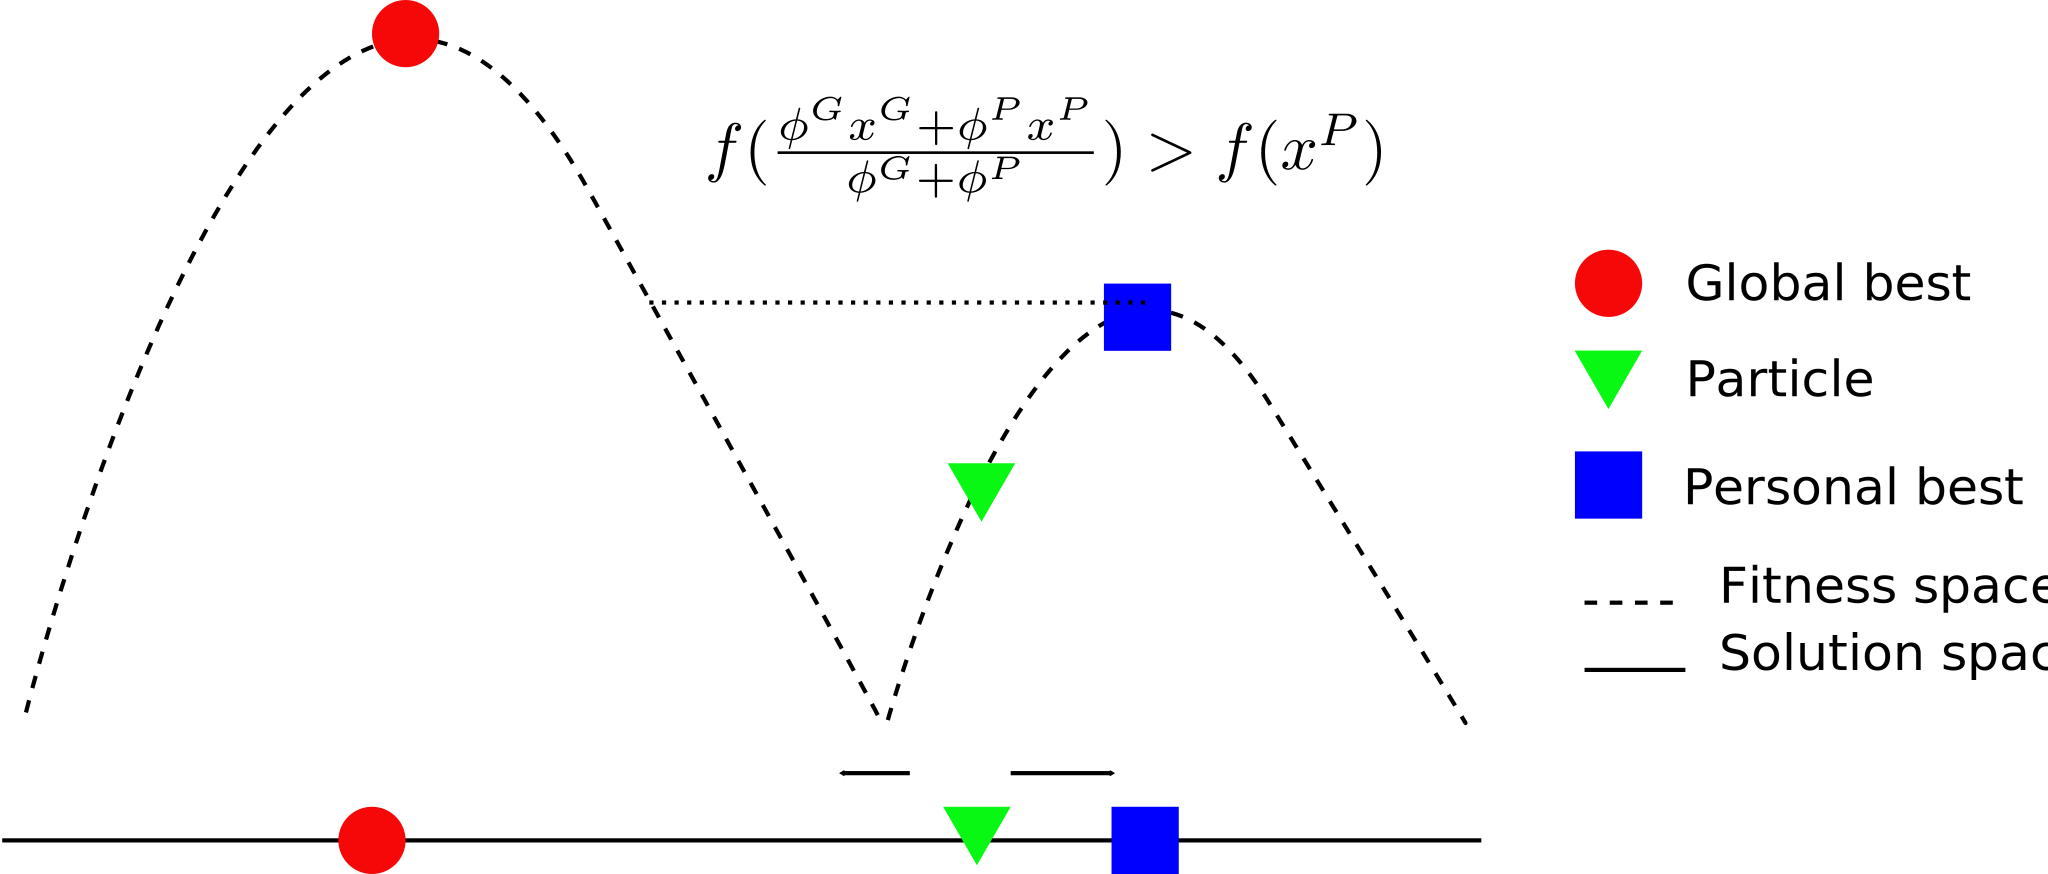
\includegraphics[width=0.9\linewidth]{./two_hills_case}
\caption{Two hills case}
\label{fig:two_hills_case}
\end{figure}





\end{document}